\documentclass[12pt,twoside,a4paper,parskip]{scrbook}
\usepackage[utf8]{inputenc}
\usepackage{csquotes}
%\usepackage[ngerman]{babel}
\usepackage{floatflt}
\usepackage{subfigure}
\usepackage[pdftex]{graphicx}
\usepackage[hidelinks]{hyperref}
\usepackage{color}
\usepackage{amssymb}
\usepackage{textcomp}
\usepackage{nicefrac}
\usepackage{scrhack}
\usepackage{pdfpages}
\usepackage{float}
\usepackage{pdflscape}
\usepackage{subfigure}
\usepackage{pdfpages}
\usepackage[verbose]{placeins}
\usepackage[nouppercase,headsepline,plainfootsepline]{scrpage2}
\usepackage{listings}
\usepackage{xcolor}
\usepackage{color}
\usepackage{caption}
\usepackage{subfigure}
\usepackage{epstopdf}
\usepackage{longtable}
\usepackage{setspace}
\usepackage{booktabs}
\usepackage[
backend=biber,
style=apa,
citestyle=authoryear-comp
]{biblatex}

\bibliography{bibliography}


%% Schauen ob die Reihenfolge passt

%%%%%%%%%%%%%%%%%%%
%% definitions
%%%%%%%%%%%%%%%%%%%
\def\BaAuthor{Achim Winter}
\def\BaAuthorStudyProgram{Computer Science}
\def\BaType{Bachelor thesis} %% passt das so?
\def\BaTitle{Operating a Smartphone as a Hardware Security Module}
\def\BaSupervisorOne{Prof.\ Dr.\ Junker-Schilling}
\def\BaSupervisorTwo{Prof.\ Dr.\ Huffstadt}
\def\BaDeadline{\today}

\ifdefined\iswithfullname
  \def\ShowBaAuthor{\BaAuthor}
\else
  \def\ShowBaAuthor{N.~N.}
\fi

\hypersetup{
pdfauthor={\ShowBaAuthor},
pdftitle={\BaTitle},
pdfsubject={Subject},
pdfkeywords={Keywords}
}

%%%%%%%%%%%%%%%%%%%
%% configs to include
%%%%%%%%%%%%%%%%%%%
\colorlet{punct}{red!60!black}
\definecolor{background}{HTML}{EEEEEE}
\definecolor{delim}{RGB}{20,105,176}
\colorlet{numb}{magenta!60!black}

\definecolor{gray}{rgb}{0.4,0.4,0.4}
\definecolor{darkblue}{rgb}{0.0,0.0,0.6}
\definecolor{cyan}{rgb}{0.0,0.6,0.6}

\definecolor{pblue}{rgb}{0.13,0.13,1}
\definecolor{pgreen}{rgb}{0,0.5,0}
\definecolor{pred}{rgb}{0.9,0,0}
\definecolor{pgrey}{rgb}{0.46,0.45,0.48}

\lstset{
  basicstyle=\ttfamily,
  columns=fullflexible,
  showstringspaces=false,
  commentstyle=\color{gray}\upshape
  linewidth=\textwidth
}

\lstdefinelanguage{json}{
    basicstyle=\normalfont\ttfamily,
    numbers=left,
    numberstyle=\scriptsize,
    stepnumber=1,
    numbersep=8pt,
    showstringspaces=false,
    breaklines=true,
    backgroundcolor=\color{background},
    literate=
     *{0}{{{\color{numb}0}}}{1}
      {1}{{{\color{numb}1}}}{1}
      {2}{{{\color{numb}2}}}{1}
      {3}{{{\color{numb}3}}}{1}
      {4}{{{\color{numb}4}}}{1}
      {5}{{{\color{numb}5}}}{1}
      {6}{{{\color{numb}6}}}{1}
      {7}{{{\color{numb}7}}}{1}
      {8}{{{\color{numb}8}}}{1}
      {9}{{{\color{numb}9}}}{1}
      {:}{{{\color{punct}{:}}}}{1}
      {,}{{{\color{punct}{,}}}}{1}
      {\{}{{{\color{delim}{\{}}}}{1}
      {\}}{{{\color{delim}{\}}}}}{1}
      {[}{{{\color{delim}{[}}}}{1}
      {]}{{{\color{delim}{]}}}}{1},
}

\lstset{language=xml,
  morestring=[b]",
  morestring=[s]{>}{<},
  morecomment=[s]{<?}{?>},
  stringstyle=\color{black},
  numbers=left,
  numberstyle=\scriptsize,
  stepnumber=1,
  numbersep=8pt,
  identifierstyle=\color{darkblue},
  keywordstyle=\color{cyan},
  backgroundcolor=\color{background},
  morekeywords={xmlns,version,type}% list your attributes here
}

\lstset{language=Java,
  showspaces=false,
  showtabs=false,
  tabsize=4,
  breaklines=true,
  keepspaces=true,
  numbers=left,
  numberstyle=\scriptsize,
  stepnumber=1,
  numbersep=8pt,
  showstringspaces=false,
  breakatwhitespace=true,
  commentstyle=\color{pgreen},
  keywordstyle=\color{pblue},
  stringstyle=\color{pred},
  basicstyle=\ttfamily,
  backgroundcolor=\color{background},
%  moredelim=[il][\textcolor{pgrey}]{$$},
%  moredelim=[is][\textcolor{pgrey}]{\%\%}{\%\%}
}

\newcommand*{\forcetwosidetitle}[1][1]{%
 \begingroup
   \cleardoubleoddpage
   \KOMAoptions{titlepage=true}% useful e.g. for scrartcl
   \csname @twosidetrue\endcsname
   \maketitle[{#1}]
 \endgroup
}


\begin{document}


%%%%%%%%%%%%%%%%%%%
%% Titelseite
%%%%%%%%%%%%%%%%%%%


\frontmatter
\titlehead{%  {\centering Seitenkopf}
  {University of applied Sciences W\"{u}rzburg-Schweinfurt\\
   Faculty of Computer Science und Business Informatics}}
\subject{\BaType}
\title{\BaTitle\\[15mm]}
\subtitle{\normalsize{submitted to the University of Applied Sciences W\"{u}rzburg-Schweinfurt in the Faculty of \BaAuthorStudyProgram}}
\author{\ShowBaAuthor}
\date{\normalsize{Submitted on: \BaDeadline}}
\publishers{
  \normalsize{First Supervisor: \BaSupervisorOne}\\
  \normalsize{Second Supervisor: \BaSupervisorTwo}\\
}
%\lowertitleback{
%\centering
\includegraphics[width=4cm]{barcode_default}

%}
\forcetwosidetitle


%%%%%%%%%%%%%%%%%%%
%% abstract
%%%%%%%%%%%%%%%%%%%

\section*{Summary}
TODO

\section*{Abstract}

TODO

\newpage
\chapter*{Acknowledgement}

I would like to thank Prof. Dr. Junker-Schilling for his helpful support. The seminars and the discussions with the other students helped me a lot to stay on schedule and make the work what it is now. My further thanks go to Prof. Dr. Huffstadt for the second correction. 

I would also like to thank Francis Pouatcha and Steffen Blümm for their support from adorsys. The discussions always brought new ideas on how the work can be further improved. Thank you very much for that.

I would also like to thank my proofreaders and my family. Thanks to you too, the work has become what it is today.

%%%%%%%%%%%%%%%%%%%
%% Inhaltsverzeichnis
%%%%%%%%%%%%%%%%%%%
\tableofcontents



%%%%%%%%%%%%%%%%%%%
%% Main part of the thesis
%%%%%%%%%%%%%%%%%%%
\mainmatter

\chapter{Introduction}\label{ch:intro}

The two main fields of cryptography in computer systems can be divided between symmetric-key cryptography and public-key cryptography. Symmetric-key utilizes the same key for the sender and the receiver, which was the first form of encryption and also secure and easy to understand. If this is done by close relatives this may be possible, but exchanging this key to every website when browsing through the internet is impractical. Not only because it is physically nearly impossible, but also because the amount of keys one would have to store securely would be growing by the square of number of communication partners.
% Maybe a picture for symmetric encryption
To avoid this kind of key management, Whitfield Diffie and Martin Hellman published a system in 1976 known as the public-key cryptography. With this system it is possible to generate an encryption key over an insecure network such as the Internet in order to secure subsequent communication. However, the real encryption key is never transferred to the opposing communication partner. In fact the real encryption key is being calculated by using public and private keys, which have a mathematical relation to each other. Each communication partner has to create a pair of his own private and public key. While the public key can be exposed to the Internet, the private key has to remain secret. 
By using both key pairs, a common shared key can be calculated which then can be used for the encryption. This system relies on the computational complexity, such as prime factorization, which is hard to do with big numbers. 
%[Was ist der Diffie-Hellman-Schlüsselaustausch?] [https://en.wikipedia.org/wiki/Cryptography#Computer_era]

The usage of encryption when visiting a web page has grown from about 30\% in 2014 to about 80\% by the end of 2019
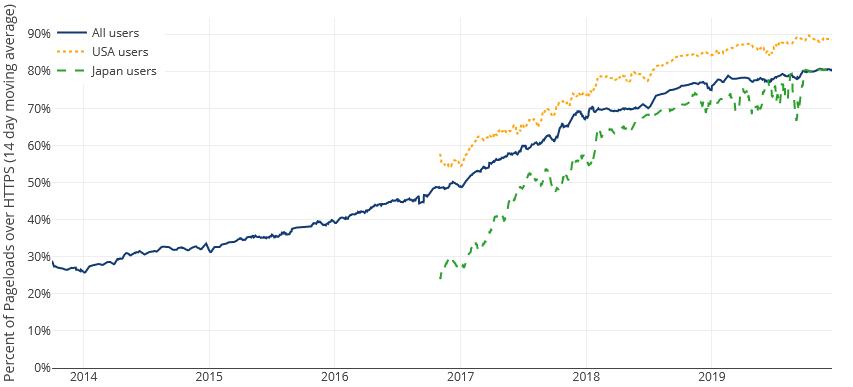
\includegraphics[Percentage of Web Pages Loaded by Firefox Using HTTPS]{ressources/https_statistics.png}
This comes due to several reasons. Whistleblower Edward Snowden has received a lot of media interest and has made people aware of using secure services on the Internet, when he revealed the capabilities of the National Security Agency (NSA). In addition, browser manufacturers like Mozilla or Google warn their users when they visit a website without HTTPS with an open red lock next to the address bar.


\section{Motivation}

The use of public/private keys is too difficult for many people, even IT professionals. The keys have to be distributed and stored securely. In many cases the distribution of keys is done by synchronizing the keys within a cloud. However, this is a potential security leak, because cloud service providers are not entirely trustworthy. On the other hand, distributing private keys
by universal serial bus (USB) is too time-consuming for many users.

\subsection{Entrepreneurial perspective}

The adorsys GmbH \& Co. KG is a software development and consulting company that specializes in the field of banking and insurance, but also develops software for industry companies. That's why internal security is especially important for adorsys and therefor also the security of communication within the company. Employees usually also have a smartphone that accesses corporate services. The management of key pairs, for example for secure email communication, is very important. 

\subsection{Social perspective}

Secure email communication is also a rarity in the private environment. Even signatures, the certainty that the person who sent me the email is really who he claims to be, is usually not given. 
One reason for this is that email communication was never developed to be secure. On the other hand, the key management and use for many is far too cumbersome. 

\section{Objective}

\section{Environment}

\section{Structural Overview}

\chapter{Approach}

\section{Analysis of the current situation}

\section{Requirements for Key-Distribution Systems}

\section{Concept}

\section{Implementation}

\chapter{Fundamentals}

\section{Quick-Response Codes}

\section{Hardware Security Module}

\section{RSA Cryptography}

\section{Secret Sharing}

Shamirs Secret Sharing. sharing keys können bei den jeweiligen PCs evtl . als Backup gelagert werden

\section{Trusted Execution Environment}

\section{Secure Element}

\section{Android Keystore System}

The Android Keystore System is a container which lets the developer store cryptographic keys without doing the en- and decryption by himself and to make it more difficult to extract the key from the device. Also, with the Keystore System, it can be authorized which app can use these keys and which not. In addition, even the apps which are authorized cannot extract the key from the device once it's stored in the Keystore System. Messages which are to be signed or encrypted are packed in a system process which carries out the cryptographic operations. Thus, an adversary would be able to use the keys if he's able to compromise an authenticated app, but never extract it on other devices.

%Another option is to use the Trusted Execution Environment or Secure Element of Android 
\subsection{Strongbox Keystore}

Since Android 9 (API Level 28), smartphones can have a Strongbox Keymaster, which relies on separated hardware and is only used for cryptographic operations.
The separated hardware always has to contain a CPU, Secure Storage, Random Key Generator and additional mechanisms to resist package tampering and unauthorized sideloading of apps.

However secrets/passwords cannot be imported in the Keystore. The ordinary way to safe information in android securely is to let the Keystore generate a Key, which then 
is safed in the keystore and is never exposed outside of the Keystore. ? 

With this generated Key you can then encrypt your own Data and safe them in the Preferences Section of your app.

\section{iOS Keychain}


\section{Signal-Protocol}

The Signal-Protocol which was developed by Open Whisper Systems for their own product, the signal messenger, is an end to end cryptography protocol used for
popular instant messaging services like Whatsapp, Facebook-Messenger or Skype. There are also a few papers which prove the security of the protocol. \parencite{cohn-gordon_formal_2017}
% Seitenzahl benoetigt wenn die komplette Arbeit daraus besteht?
\newline
The protocol uses a long-term identity key pair, a medium-term signed prekey pair and multiple transient keys, which are generated on each client and also stored there
securely.

If a client wishes to offer himself as a communication partner, he has to generate a PreKey Bundle and send it to the other communication party.
Usually this is done by uploading the bundle to a \nameref{subsec:KDC}. 

\subsection{Key Agreement Protocol}

The Key Agreement Protocol is build upon the Extended Triple Diffie-Hellman (X3DH) Protocol. By using it a shared secret key can be generated which authentication
is based upon public keys. 
% Blabla --> Providing forward secrecy and cryptographic deniability.


\subsection*{Key Distribution Center}
\label{subsec:KDC}

A Key Distribution Center is a network device with the purpose of storing and exchanging keys. Within the Signal Protocol the Key Distribution Center is used
as a trusted party where so called Pre Key Bundles are uploaded. These Bundles contain information which is needed to create a session to a communication partner.
The information contained consists of:
\begin{itemize}
  \item registrationId
  \item deviceId
  \item preKeyId
  \item PreKeyPublic
  \item signedPreKeyId
  \item signedPreKeyPublic
  \item signedPreKeySignature
  \item identityKey
\end{itemize}


% \section{Web of trust}

%\chapter{Problem definition}

\chapter{Analysis of the current situation}

\section{Usage of private keys}

\section{Distribution of private keys}

\subsection{Local/Offline}

USB or some other offline connections are used to transfer the private key.

% \subsubsection{Subkeys}

% Only possible for pgp
% Only the latest subkey can be used to encrypt messages. Thus, every device must be in possession of this subkey. 

\subsection{Webservers/Downloads}

Possible vulnerability by man in the middle attacks.
The private key is stored on a trusted server. Whenever a new device is added, the user can download his private key.

\subsection{External Providers}

Using Services like Dropbox or Google drive. This can be combined with encrypting the private key and or separating the key using secret sharing and 
storing them on different clouds. 




\chapter{Requirements for Key-Distribution Systems}

\section{Usability}

\section{Security}

Enter a passphrase on computer and then on mobile phone would add security but isn't that convenient.

%\section{Loss Coverage}
% Kommt nur in ausblick
\chapter{Concept}

\section{Architecture}

\section{Usability}

\chapter{Implementation}

\section{Kotlin}

\section{gRPC}

\section{Prototype}

\subsection{App}

\subsection{Desktop Client}

% Nach dem verbinden mit QR Code könnte in der App eine Pin angezeigt werden die dann am PC eingegeben werden muss.


\chapter{Evaluation}

\section{Usability}

\section{Security}

%\section{Existing Solutions}

%\section{QR-Based Solution}

\chapter{Summary}

\chapter{Outlook}

Backup can be implemented using social secret sharing or other things.

You could create clients for all kinds of desktop Programs, ssh, pgp, and so on.

\parencite{gamma2011patterns}

\backmatter
%%%%%%%%%%%%%%%%%%%
%% create figure list
%%%%%%%%%%%%%%%%%%%

\listoffigures
\addcontentsline{toc}{chapter}{Directories}

%%%%%%%%%%%%%%%%%%%
%% create tables list
%%%%%%%%%%%%%%%%%%%
\listoftables

%%%%%%%%%%%%%%%%%%%
%% create listings list
%%%%%%%%%%%%%%%%%%%
%\lstlistoflistings
%\addcontentsline{toc}{chapter}{Listings}

\cleardoublepage
\phantomsection
\addcontentsline{toc}{chapter}{Bibliography}
\printbibliography

%%%%%%%%%%%%%%%%%%%
%% declaration on oath
%%%%%%%%%%%%%%%%%%%

\addchap{Affidavit}

I hereby certify that I have written my bachelor thesis independently and have not yet submitted it for examination purposes elsewhere. All sources and aids used are listed, literal and meaningful quotations have been marked as such.

\vspace{20pt}
\begin{flushright}
$\overline{~~~~~~~~~~~~~~~~~\mbox{\ShowBaAuthor, am \today}~~~~~~~~~~~~~~~~~}$
\end{flushright}

\addchap{Consent to plagiarism check}

I hereby agree that my submitted work may be sent to PlagScan (www.plagscan.com) in digital form for the purpose of checking for plagiarism and that it may be temporarily (max. 5~years) stored in the database maintained by PlagScan as well as personal data which are part of this work may be stored there.

\begin{small}
This Consent is voluntary. Without this consent, the plagiarism check can still take place, when all personal data is removed from the document. Consent to the storage and use of personal data may be revoked at any time by notifying the faculty.
\end{small}

\vspace{20pt}
\begin{flushright}
$\overline{~~~~~~~~~~~~~~~~~\mbox{\ShowBaAuthor, am \today}~~~~~~~~~~~~~~~~~}$
\end{flushright}

\end{document}
